%\documentclass[12pt,xcolor=dvipsnames,mathserif]{beamer}
\documentclass[12pt,xcolor=dvipsnames,handout,mathserif,aspectratio=169]{beamer}

\usepackage{hyperref}

\usepackage{pgfpages}
%\pgfpagesuselayout{2 on 1}[border shrink=2.5mm]
%\pgfpageslogicalpageoptions{1}{border code=\pgfusepath{stroke}}
%\pgfpageslogicalpageoptions{2}{border code=\pgfusepath{stroke}}


% Specify theme
%\usetheme{Madrid}
\usetheme{Boadilla}
% See deic.uab.es/~iblanes/beamer_gallery/index_by_theme.html for other themes

% Specify base color
%\usecolortheme[named=OliveGreen]{structure}
\usecolortheme[named=RoyalBlue]{structure}
% See http://goo.gl/p0Phn for other colors

% Specify other colors and options as required
\setbeamercolor{alerted text}{fg=Red}
\setbeamertemplate{items}[square]

% Specify some useful short commands
\newcommand{\bbl}[1]{{\color{NavyBlue} \textbf{#1}}}
\newcommand{\bre}[1]{{\color{red} \textbf{#1}}}
\newcommand{\bgr}[1]{{\color{PineGreen} \textbf{#1}}}
\newcommand{\un}{\texttt{\char`_}}


% Title and author information
\title[Introductory Statistics with Excel]{Introductory Statistics with Excel}
\author[Andrew Parnell]{Andrew Parnell}
\institute[UCD]{University College Dublin \begin{center} 
\includegraphics[width=1.5cm]{UCDlogo.pdf}\end{center} }
%\date{Lecture 2 -- part 1}
\date[Class 1]{Class 1 - Basics}

\begin{document}

\titlepage

\begin{frame}{ Introduction}

In this course we will cover:
\begin{itemize}
\item Class 1: Graphical and tabular summaries of data 
\item Class 2: Basics of experimental design and probability distributions
\item Class 3: Hypothesis testing 
\item Class 4: Confidence intervals and $t$-tests
\item Class 5: Statistical modelling and ANOVA
\item Class 6: Linear regression and control charts
\end{itemize}
\vspace{0.3cm}
There are also four Excel practicals.\\
\vspace{0.3cm}
I assume you have basic mathematical ability, some experience with using Excel, but very few formulae are used in these notes

\end{frame}

\begin{frame}{ Data sets }

We will use three main data sets throughout this course:
\begin{enumerate}
\item The milk yield of 14 cows in kg
\item A genomic breeding value of cows based on a genetic marker expression level
\item A two-way unbalanced experiment on Clenbuterol based on 3 different doses over 3 different runs
\end{enumerate}
As well as a number of small ones for illustration. All are included in the \texttt{course\_data.xls} file
\end{frame}

\begin{frame}{Data set 1}

Questions:\\ 
\vspace{0.5cm}
What is the shape of the distribution of milk yield for cows?\\
\vspace{0.5cm}
Are there any outlying values?\\
\vspace{0.5cm}
Is the mean milk yield for these cows 120kg?\\
\vspace{0.5cm}
How certain can we be about the mean milk yield?\\
\end{frame}

\begin{frame}{Data set 2}

Questions:\\ 
\vspace{0.5cm}

Is there a relationship between the two variables?\\
\vspace{0.5cm}
If so, what is the shape of that relationship?\\
\vspace{0.5cm}
Is one variable causing the other to change?\\
\end{frame}

\begin{frame}{Data set 3}

Questions:\\ 
\vspace{0.5cm}
How important is the fortification?\\
\vspace{0.5cm}
Which is more variable, the runs or the replicates?

\end{frame}

\begin{frame}{ Turning data into information }

In this class we will look at:
\begin{itemize}
\item The general characteristics of data
\item Samples and populations
\item Different types of data
\item Summaries of location and scale
\item Outliers and missing data
\item Summarising data via graphics
\end{itemize}

\end{frame}

\begin{frame}{ Raw data }

Often, we are first presented with \bre{raw data}, e.g.:
\begin{table}[ht]
\centering
\begin{tabular}{rrr}
  \hline
 & Expression & Breeding value \\ 
  \hline
1 & 1.58 & 5.43 \\ 
  2 & 0.09 & 3.54 \\ 
  3 & 0.82 & 5.14 \\ 
  4 & 0.58 & 3.60 \\ 
  5 & 1.91 & 8.07 \\ 
  6 & 1.88 & 6.91 \\ 
  \vdots & \vdots & \vdots \\ 
   \hline
\end{tabular}
\end{table}\pause
The raw data is where we always start. We need to turn it into useful information.\\
\pause
\vspace{0.2cm}

\end{frame}

\begin{frame}{ Observations and variables }

\begin{itemize}
\item An \bgr{observation} is a set of answers on a single unit, such as a cow or a person. In the previous slide the expression and breeding value of a single cow constitute one observation
\pause
\item A \bgr{variable} is a single characteristic of a set of observations, such as the breeding value
\end{itemize}
\pause
We traditionally arrange the data set so that the observations make up the rows of a table and the variables make up the columns.\\
\vspace{0.5cm}
The number of observations is referred to as the sample size, often represented by the letter $n$, e.g. $n=120$.
\end{frame}

\begin{frame}{ Samples and populations }

We will usually use \bbl{sample} data to make inferences about the larger \bre{population} represented by the data. When data are collected from all the members of a population it is called a \bgr{census}. Most commonly, a census is too expensive to conduct.\\
\pause
\vspace{0.2cm}
The distinction between a sample and a population can be unclear. If we are only interested in the cows at one particular farm then we have just conducted a \bgr{census}. If we are interested in learning about a larger population (e.g. all cows, or all Irish cows) then we have a \bbl{sample}. \\
\end{frame}

\begin{frame}{ Parameters and statistics }

A summary measure created from the raw sample data is called a \bgr{statistic}. A summary measure from an entire population is called a \bbl{parameter}.\\
\pause
\vspace{0.2cm}
Most often, we are interested in estimating the \bbl{parameters} from sample data. We try to create \bgr{statistics} which are good estimators of the parameters
\end{frame}

\begin{frame}{ Types of variable }

There are generally three types of variable: \bbl{categorical}, \bgr{ordinal}, and \bre{quantitative}. Some examples:
\small
\begin{center}
\begin{tabular}{p{4cm}|p{4.5cm}|l}
\hline
\hline
Variable & Possible Answers & Variable Type \\
\hline
\hline
Height in cm & Measured height in cm & Quantitative \\
\hline
Tenderness rating & 1=Poor,..., 10=Excellent & Ordinal \\
\hline
Sex & Male or Female & Categorical \\
\hline
\vdots & \vdots & \vdots \\
\hline
\hline
\end{tabular}
\end{center}
\only<5>{
Not all numbers are quantitative variables (e.g. your telephone number)}
\end{frame}

\begin{frame}[fragile]{}
\bbl{\Huge Summarising categorial and ordinal data}\\ 
\vspace{0.5cm}
\end{frame}

\begin{frame}{ Summarising categorical variables }

Categorical and ordinal variables can be summarised in a \bbl{frequency} or \bbl{relative frequency} table. A frequency table gives just the counts of the data whilst the relative frequencies give the percentages.\\
\pause
\vspace{0.2cm}
Example: seat-belt use by 18 year olds
\begin{center}
\begin{tabular}{lrr}
\hline
\hline
Response & \centering Frequency & Relative Frequency \\
 & (Count) & (Percentage) \\
\hline
Always & 1686 & 55.4\% \\
Most times & 578 & 19.0\% \\
Sometimes & 414 & 13.6\% \\
Rarely & 249 & 8.2\% \\
Never & 115 & 3.8\% \\
\hline
Total & 3042 & 100.0\% \\
\hline
\hline
\end{tabular}
\end{center}
\end{frame}

\begin{frame}{ Summarising categorical variables 2 }

When there is more than one categorical/ordinal variable, we can use a cross-tabulation\\
\pause
\vspace{0.2cm}
Example: seat-belt use by 18 year olds
\scriptsize
\begin{center}
\begin{tabular}{lrrrrrr}
\hline
 & Always & Most Times & Sometimes & Rarely & Never & Total \\
 \hline
 Female & 915 & 276 & 167 & 84 & 25 & 1467 \\
 & (62.4\%) & (18.8\%) & (11.4\%) & (5.7\%) & (1.7\%) & (100\%) \\
 \hline
 Male & 771 & 302 & 247 & 165 & 90 & 1575 \\
 & (49.0\%) & (19.2\%) & (15.7\%) & (10.5\%) & (5.7\%) & (100\%) \\
 \hline
\end{tabular}
\end{center}
\pause
\normalsize
Often, the relative frequencies are more informative as they account for the sample size \\
\pause
\vspace{0.2cm}
Categorical/Ordinal variables can be summarised numerically by the \bbl{mode}; the category with the highest frequency. For males and females in this example the mode is the category `Always'.
\end{frame}

\begin{frame}{ Summarising quantitative variables: location }

The following are all way summarising the \bbl{central location} of the data:
\vspace{0.5cm}
\begin{description}
\item[Means] Computed by adding together all the values of a variable and dividing by the sample size. 
\item[Medians] Computed by placing the data in size order and finding the middle value
\item[Quartiles] Computed by placing the data in size order and finding the values 25\% and 75\% of the way through
\end{description}
\begin{block}{}
Whilst the mean, median and the mode are all forms of \bgr{average}, Excel uses the function \texttt{average} to compute only the mean.
\end{block}
\end{frame}

\begin{frame}{Example: finding means and medians}

Our 14 cows' milk yields were :\\
\texttt{101.7 103.3 111.6 113.2 123.4 130.9 142 143.5 146.1 155.1 155.5 169.3 169.6 170.7}\\
\pause
To find the mean we compute:\\
\tiny
\begin{eqnarray*}
\mbox{mean} &=& \frac{169.6 + 142 + 103.3 + 111.6 + 123.4 + 143.5 + 155.1 + 101.7 + 170.7 + 113.2 + 130.9 + 146.1 + 169.3 + 155.5}{14}\\
 &=& \frac{1935.9}{14} =  138.3\mbox{ kg}
\end{eqnarray*}
\normalsize
\pause
For the median we do not have a middle value so we find the mean of the 7th and 8th values giving:
$$\mbox{median} = \frac{142 + 143.5}{2} = 142.75\mbox{ kg}$$
\pause
What can we say about the difference between the mean and median here?
\end{frame}

\begin{frame}{ Example 2: CEO pay }
The top 7 salaries of the highest paid CEOs in the US in 2009 was:\\
\$556m (LJ Ellison; Oracle), \$222m (RR Irani; Occidental Petroleum), \$154m (JB Hess; Hess), \$116m (MD Watford; Ultra Petroleum), \$90m (MG Papa; EOG Resources), \$87m (WR Berkley; WR Berkley), \$68m (MK Rose; Burlington Santa)\\
\vspace{0.2cm}
\pause
The mean is now:
$$\mbox{mean} = \frac{556 + 222 + 154 + 116 + 90 + 87 + 68}{7} = \$184.7\mbox{m}$$
and the median:
$$ \mbox{median} = \$116\mbox{m}$$
\pause
Why are the mean and the median different here?
\end{frame}

\begin{frame}{ Some notes about means and medians }

\begin{itemize}
\item The mean is much more sensitive to \bre{outliers}: extreme observations. It is easy for it do be dragged up and down
\pause
\item The median is much more \bgr{robust}, however it does not have as many nice theoretical properties as the mean (see later classes on sampling distributions)
\pause
\item Often raw data are given as \bbl{codes}, e.g. Male = 0, Female = 1, so that the mean of this variable represents the proportion of Females in the sample. You need to be careful that the codes are set correctly for this to work. For example, if Male = 1 and Female = 2, the mean is going to be meaningless! 
\pause
\item Modes are generally not calculated for quantitative variables until a \textbf{probability distribution} (see later classes) is assumed for the data
\end{itemize}

\end{frame}

\begin{frame}{Summarising quantitative variables: scale }

\begin{itemize}
\item The scale or spread of a quantitative variable is usually represented by the \bbl{variance/standard deviation}, the \bgr{range} or the \bre{inter-quartile range (IQR)}
\pause
\item The \bgr{range} is simply the maximum value minus the minimum
\pause
\item The \bre{IQR} is the difference between the upper quartile and the lower quartile
\pause
\item The \bbl{variance} is the sum of squared deviations from the mean, divided by the sample size minus 1. The \bbl{standard deviation} is the square root of the variance
\pause
\item As before, the \bbl{variance} is more affected by outliers than the \bre{IQR}, but has nicer theoretical properties
\end{itemize}
\pause
\end{frame}

\begin{frame}{ Example: milk yields }

\begin{itemize}
\item Going back to the cow data we have:\\
\texttt{101.7 103.3 111.6 113.2 123.4 130.9 142 143.5 146.1 155.1 155.5 169.3 169.6 170.7}\\

\pause
\item The range is $170.7 - 101.7 = 69$kg
\pause
\item The quartiles are 115.75 and 155.40 so the IQR = $155.40 - 115.75 = 39.6$kg
\pause
\item The mean was 138.3 so the variance can be calculated as:
\scriptsize
$$(\mbox{standard deviation})^{2} = \frac{ (101.7 - 138.3)^{2} + (103.3 - 138.3)^{2} + \ldots + (170.7-138.3)^{2} }{ 14 - 1} = 604.18\mbox{ (kg)$^2$}$$
\normalsize
\pause
\vspace{-0.3cm}
\item And the standard deviation as:
$$\sqrt{\mbox{variance}} = \sqrt{604.18} = 24.58\mbox{mph}$$
\end{itemize}
\end{frame}

\begin{frame}{Some details about measures of scale}
\begin{itemize}
\item Note that the range, the IQR, and the standard deviation are all in the \bbl{original} units (e.g. kilograms), whereas the variance is in \bre{squared} units, so is often not as helpful to report
\pause
\item In the variance calculation we divide by $n-1$ so as to get an \bgr{unbiased} estimator of the population variance
\item It's hard to interpret a standard deviation value by itself. It's often more useful to compare the standard deviations across different groups
\end{itemize}
\end{frame}

\begin{frame}{Outliers }

An \bre{outlier} is an extreme or unusual observation. Common scenarios are:
\begin{itemize}
\item \bgr{It is a legitimate data value and represents the natural variability for the variable(s) measured.} In this case we should not remove it as it provides important information about the data
\pause
\item \bbl{A mistake was made in taking the measurement.} In this case we should check with the experimenter before discarding or ignoring it
\pause
\item \bre{The observation actually belongs to a different population.} In this case it should either be discarded or the study re-run to include more samples from the wider population
\end{itemize}
\end{frame}

\begin{frame}[fragile]{}
\bbl{\Huge Statistical graphics}\\ 
\vspace{0.5cm}
\end{frame}

\begin{frame}{ Statistical graphics  }

\begin{block}{}
Drawing graphs from data is one of the most \bbl{important} and \bre{under-rated} parts of statistics
\end{block}
\pause
\vspace{0.2cm}
A well-structured and suitably labelled graph can summarise a variable (or set of variables) far more efficiently than any other format\\

\end{frame}

\begin{frame}{ Producing graphs: golden rules }

\begin{itemize}
\item A graph should be self-explanatory, so that the reader does not need any further information to understand what is going on
\pause
\item There should always be clear labels on the vertical ($y$) axis and the horizontal ($x$) axis
\pause
\item If necessary, include a caption beneath or above the plot that explains what the graph is showing
\pause
\item Add extra touches, such as grid lines, colours, different point styles, etc, if they make the plot easier to understand.
\end{itemize}
\pause
Creating a good graph looks easy but requires a lot of thought and is actually very hard!
\end{frame}

\begin{frame}{ Bar charts and histograms  }

\begin{itemize}
\item Bar charts and histograms might look alike but they are very different. 
\pause
\item Bar charts are used on the frequencies of categorical or ordinal variables. Histograms are used on quantitative variables only 
\pause
\item Bar charts are very simple to create. They height of the bar represents the frequency or relative frequency of that category.\\
\pause
\item Histograms are a bit more complicated:
\begin{enumerate}
\item Decide on a number of cut-off points or bins
\item Count the number of observations within each bin. 
\item The height of the bar is the count (or relative count) inside each bin.
\end{enumerate}
\end{itemize}
\end{frame}

\begin{frame}{ Example bar chart }

\begin{center}
\includegraphics[width=0.7\textwidth]{SeatbeltBarChartCompare.pdf}
\end{center}

\end{frame}


\begin{frame}{ Bar charts 2 }

Some considerations:
\begin{itemize}
\item Bar charts can be horizontal as well as vertical, which can sometimes make them easier to read
\pause
\item If using relative frequencies, it can sometimes be helpful to `stack' the bars on top of each other so they total 100\%
\pause
\item Use grid-lines if necessary so that the reader can clearly see the differences between different bar heights
\end{itemize}

\end{frame}

\begin{frame}{ Creating a histogram }

Some data on driving speeds:\\
\texttt{61 64 66 70 71 71 74 75 76 82 83 86 86 87 89 89 92 92 92 92 92 93 93 94 94 96 97 98 98 99 99 99 100 102 102 104 104 104 105 105 106 107 107 108 108 109 110 111 112 113 113 114 116 
116 117 118 119 119 120 120 122 124 125 125 126 128 129 130 130 130 131 132 133 136 136 142 142 143 146 146 148 149 150 150 151 151 152}\\
\pause
Suppose we set the bins at\\ \texttt{60-70, 71-80, ..., 141-150, 151-160}.\\
\vspace{0.2cm}
We would obtain frequencies of:
\tiny
\begin{center}
\begin{tabular}{cccccccccc}
\hline
61-70 & 71-80 & 81-90 & 91-100 & 101-110 & 111-120 & 121-130 & 131-140 & 141-150 & 151-160\\
\hline
4 & 5 & 7 & 17 & 14 & 13 & 10 &  5 &  9 &  3 \\
\hline
\end{tabular}
\end{center}

\end{frame}

\begin{frame}{ Example histogram }
\begin{center}
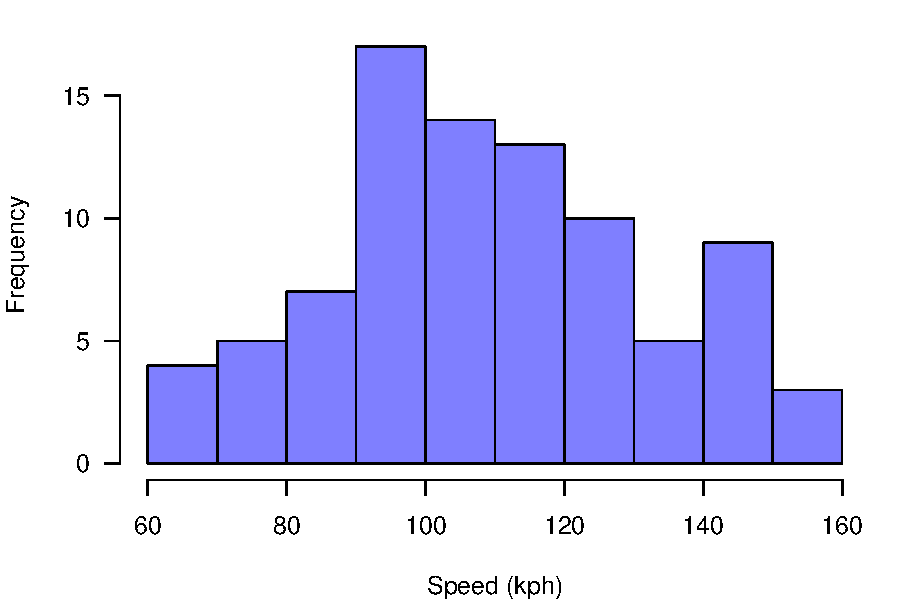
\includegraphics[width=0.7\textwidth]{MaleSpeedHist.pdf}
\end{center}


\end{frame}

\begin{frame}{ Considerations in drawing histograms }

\begin{itemize}
\item Choosing the number/size of bins is very important. If you choose \bre{too many narrow} bins the histogram will look very bumpy. If you choose \bre{too few fat} bins then some of the interesting features will be lost
\pause
\item Multiple histograms on top of each other can be useful in determining the differences between two groups
\pause
\item From a histogram it can be easy to spot \bgr{skew}, whereby values are more spread out on one side of the graph than the other. If a graph is not skewed it is described as \bbl{symmetric}
\end{itemize}

\end{frame}

\begin{frame}{ Box plots  }

Box plots (or Box and whisker plots) are a very neat way of comparing multiple groups side-by-side.
\vspace{-1cm}
\begin{center}
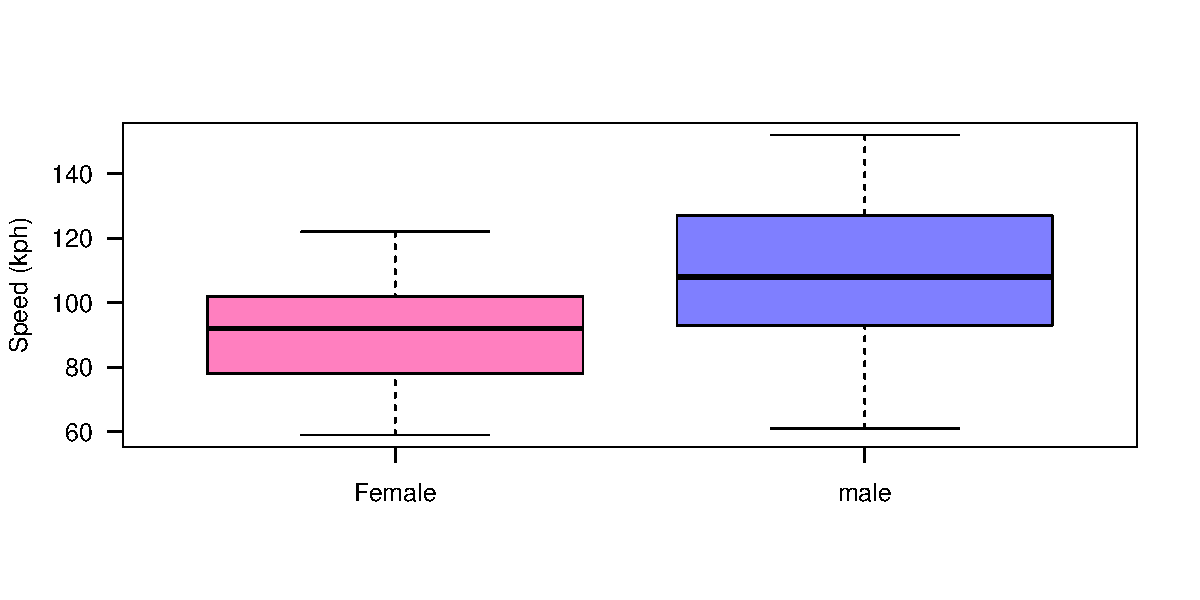
\includegraphics[width=0.7\textwidth]{SpeedBoxplots.pdf}
\end{center}
\vspace{-1cm}
The central line is the median, whilst the edges of the box are the quartiles, and the whiskers are the extremes.\\
\pause
\begin{block}{}
The collection of the median, quartiles and extremes is sometimes called the \bgr{five number summary}.
\end{block}
\end{frame}

\begin{frame}{ Pie charts }

Pie charts a waste of time. Do not create pie charts.
\begin{center}
\begin{tabular}{cc}
\hspace{-1cm} 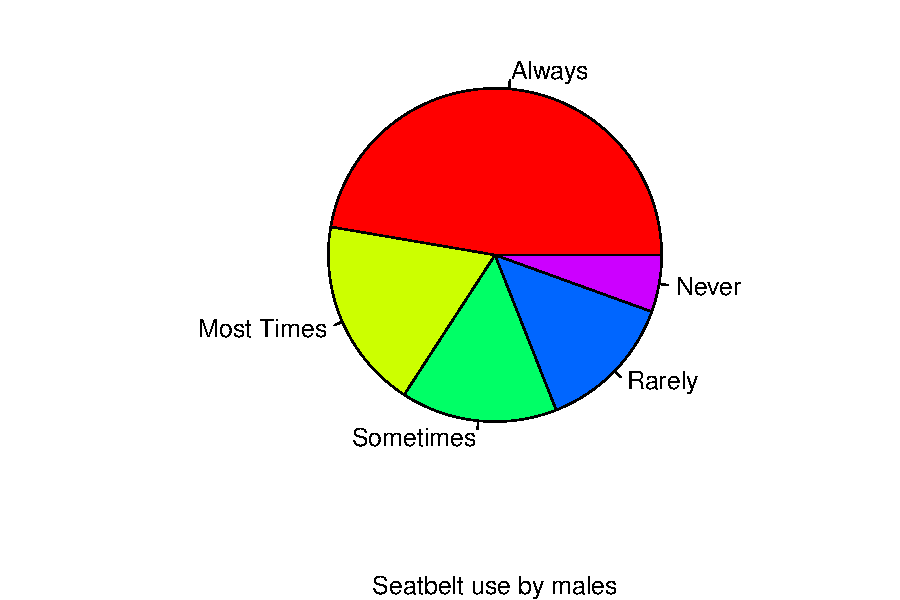
\includegraphics[width=0.6\textwidth]{SeatBeltPieChartCompare.pdf} & \hspace{-1cm} 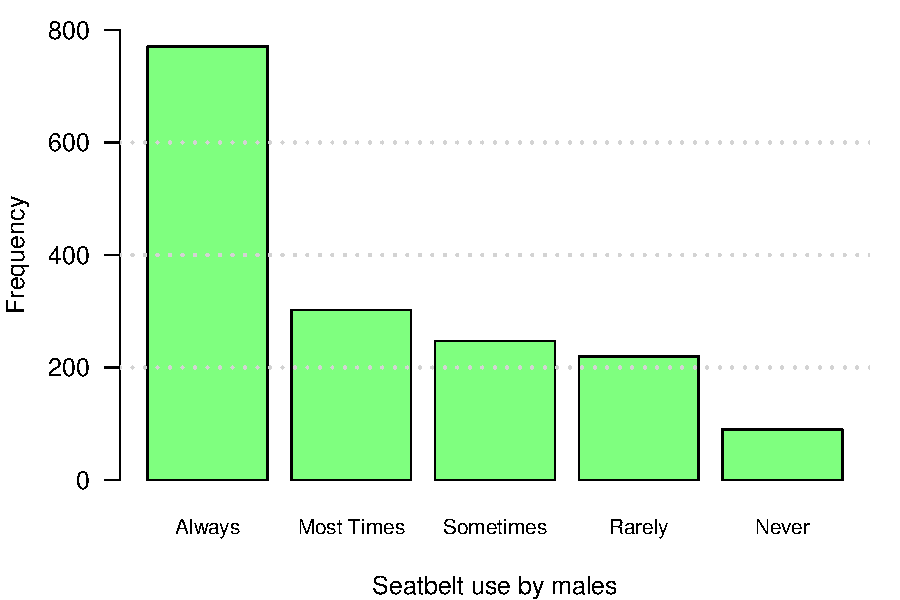
\includegraphics[width=0.5\textwidth]{SeatBeltBarChartCompare.pdf} \\
\end{tabular}
\end{center}

\end{frame}

\begin{frame}{ The classic }

\begin{center}
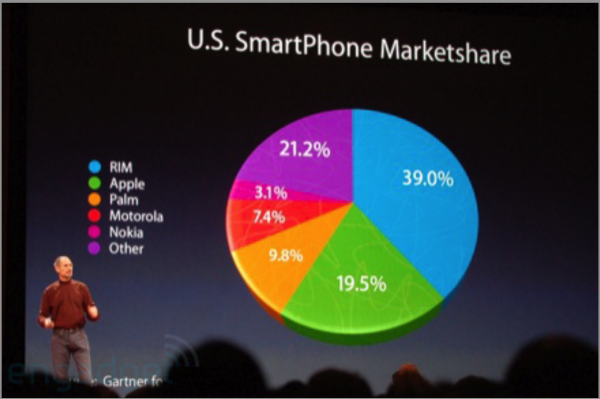
\includegraphics[width=0.7\textwidth]{apple.png}
\end{center}

\end{frame}

\begin{frame}{ But... }

Similar to a pie chart, yet a bit more useful, is a rose plot. The following represents wind speed at Dublin airport:
\begin{center}
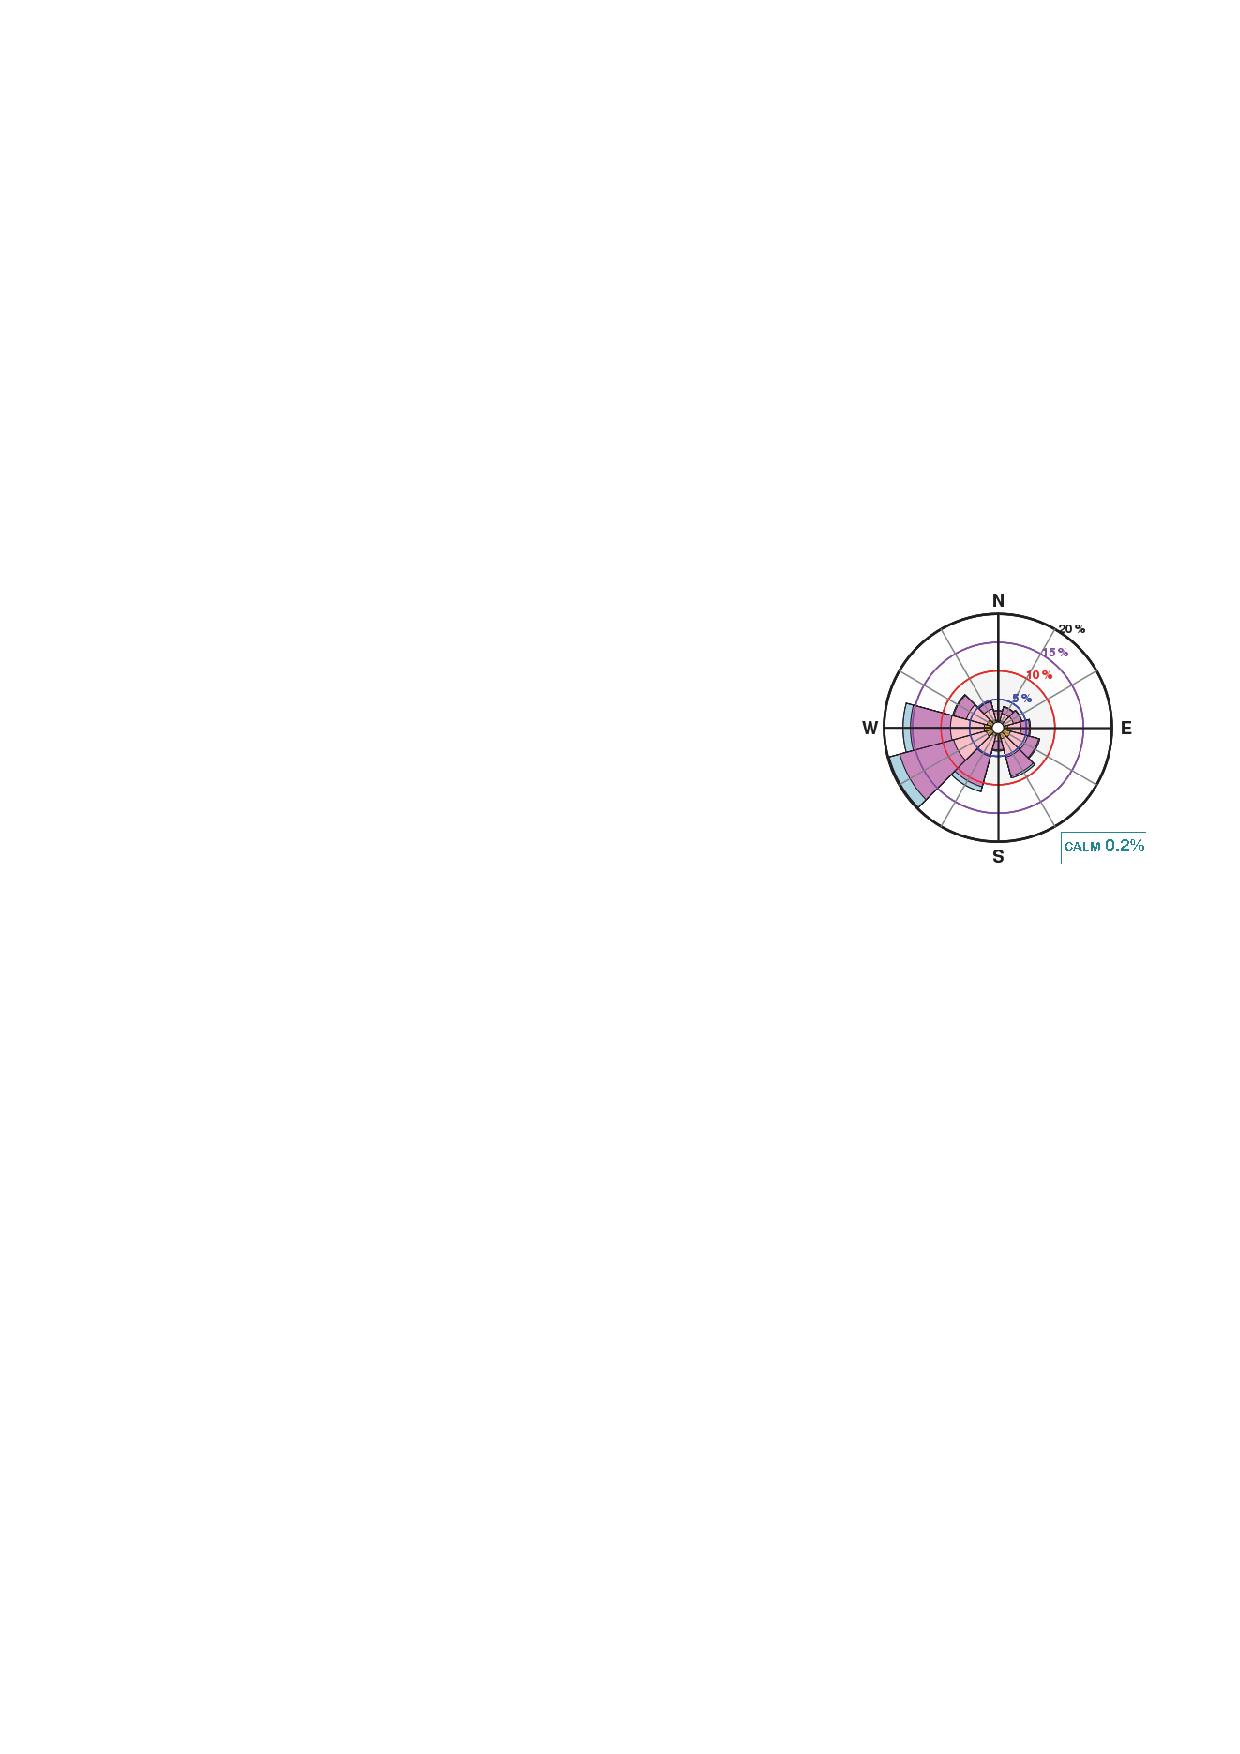
\includegraphics[width=0.4\textwidth]{GoodPieChart.pdf}
\end{center}

\end{frame}


\begin{frame}{ Scatter plots }

The neatest way to represent two quantitative variables simultaneously is a scatter plot. 
\begin{center}
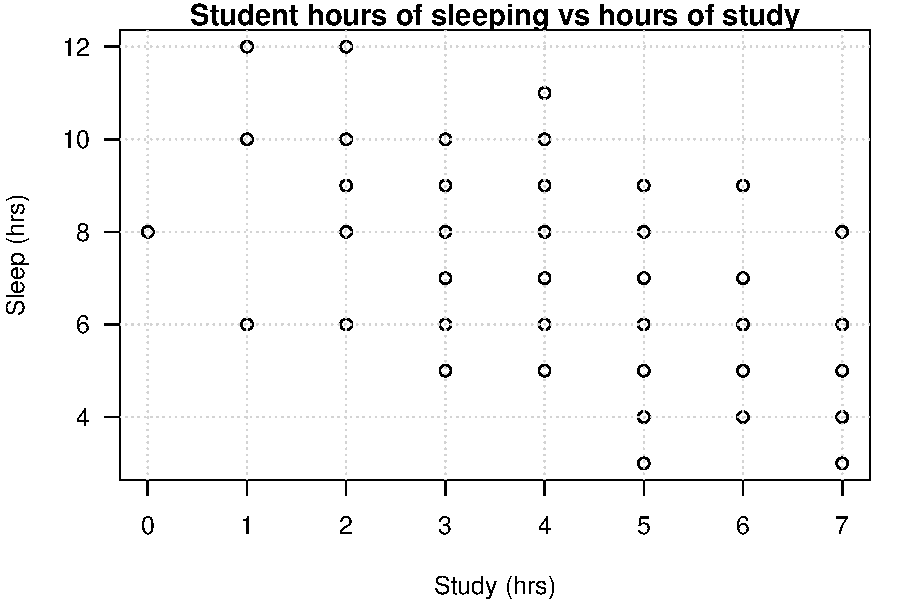
\includegraphics[width=0.5\textwidth]{StudySleepScatter.pdf}
\end{center}
\pause
Each observation is a point on the graph, e.g. hrs of study = 6, hrs of sleep = 8.

\end{frame}

\begin{frame}{ Line plots  }

If a scatter plot has a natural ordering in the $x$-axis, it is usual to join the points to create a line plot:
\begin{center}
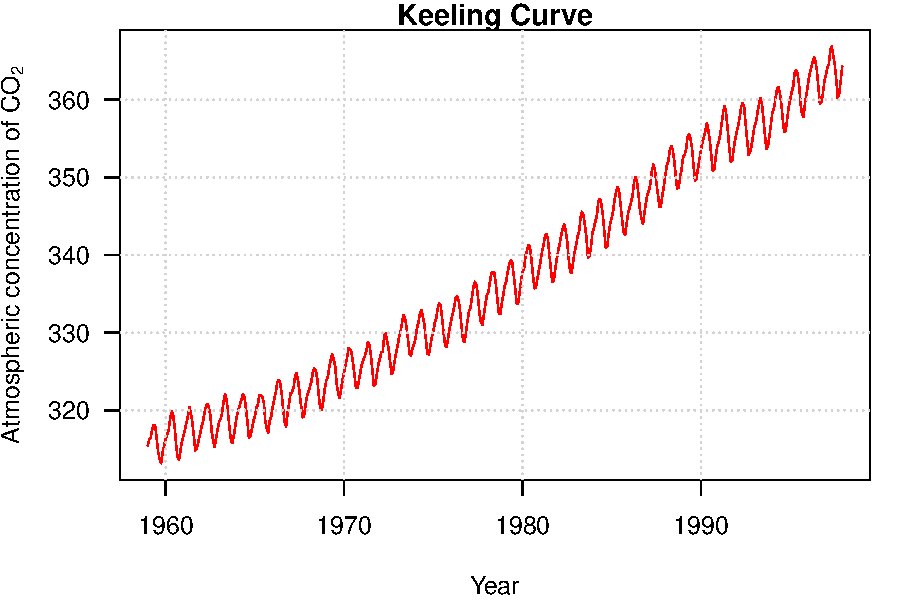
\includegraphics[width=0.7\textwidth]{KeelingCurve.pdf}
\end{center}

\end{frame}

\begin{frame}{ Class 1 summary  }

\begin{itemize}
\item Always think about \bbl{populations/samples}, and \bgr{parameters/statistics}
\item Summarise data with measures of \bbl{location} (mean/median/mode) and \bgr{scale} (standard deviation, inter-quartile range)
\item Use statistical graphics \bbl{carefully} and \bgr{thoughtfully} to present your data
\end{itemize}


\end{frame}


\end{document}